% Gemini theme
% https://github.com/anishathalye/gemini
%
% We try to keep this Overleaf template in sync with the canonical source on
% GitHub, but it's recommended that you obtain the template directly from
% GitHub to ensure that you are using the latest version.

\documentclass[final]{beamer}

% ====================
% Packages
% ====================
\usepackage{graphicx}
\usepackage[T1]{fontenc}
\usepackage{lmodern}
\usepackage[size=custom,width=120,height=72,scale=1.0]{beamerposter}
\usetheme{gemini}
\usecolortheme{gemini}
\usepackage{graphicx}
\usepackage{booktabs}
\usepackage{tikz}
\usepackage{pgfplots}
\pgfplotsset{compat=1.14}
\usepackage{fontspec}
\setmainfont{Times New Roman}
% ====================
% Lengths
% ====================

% If you have N columns, choose \sepwidth and \colwidth such that
% (N+1)*\sepwidth + N*\colwidth = \paperwidth
\newlength{\sepwidth}
\newlength{\colwidth}
\setlength{\sepwidth}{0.025\paperwidth}
\setlength{\colwidth}{0.3\paperwidth}

\newcommand{\separatorcolumn}{\begin{column}{\sepwidth}\end{column}}

% ====================
% Title
% ====================

\title{Quantitative trading based on AlphaNet}

%\author{ \and  }


% ====================
% Footer (optional)
% ====================

\footercontent{
  \href{}{} \hfill
   \hfill
  \href{}{}}
% (can be left out to remove footer)

% ====================
% Logo (optional)
% ====================

% use this to include logos on the left and/or right side of the header:
% \logoright{\includegraphics[height=7cm]{logo1.pdf}}
% \logoleft{\includegraphics[height=7cm]{logo2.pdf}}

% ====================
% Body
% ====================

\begin{document}

\begin{frame}[t]
\begin{columns}[t]
\separatorcolumn

\begin{column}{\colwidth}

  \begin{block}{\Large Abstract}

    \large \textmd{Inspired by the CNN and RNN, we propose a new quantitative trading model. This model overcomes the problem of poor performance of traditional convolutional network models on time series, especially financial data series, by combining GRU and transformer with CNN model. We get good prediction results on the SP&100 dataset after 2015.}

  \end{block}
    
  \begin{block}{\Large Motivation}
    \large \textmd{The key to the success of our model is to combine the convolutional network and the sequence model. Since CNN is used to extract features in image classification, and RNN can learn the relationship in time, we think that we can transform financial data into "data picture", input them into CNN to extract features and use sequence model makes predictions.}
  \end{block}

  \begin{alertblock}{Methods}
    \begin{itemize}
      \item \textbf{CNN} Use the data image as the input to the CNN. The data for each stock forms a data image from $t - n$ to $t$. If we have n stocks in an interval, we can get n images of the data for that interval. In the data image, each column represents a time step (such as a day), and different rows represent different types of values. Such as opening price, highest price, lowest price, closing price, one-day yield, etc.
        \\ \hspace*{\fill} \\
      \begin{center}
      \begin{tabular}{|c|c|c|c|}% 通过添加 | 来表示是否需要绘制竖线
    \hline  % 在表格最上方绘制横线
    $open(t-n)$&$...$&$open(t-1)$&$open(t)$\\
    \hline  
    $high(t-n)$&$...$&$high(t-1)$&$high(t)$\\
    \hline  
    $low(t-n)$&$...$&$low(t-1)$&$low(t)$\\
    \hline  
    $close(t-n)$&$...$&$close(t-1)$&$close(t)$\\
    \hline  
    $volume(t-n)$&$...$&$volume(t-1)$&$volume(t)$\\
    \hline  
    \multicolumn{4}{|c|}{Some other features}\\
    \hline % 在表格最下方绘制横线
    \end{tabular}
    \end{center}
    \\ \hspace*{\fill} \\
\begin{figure}
  \centering
  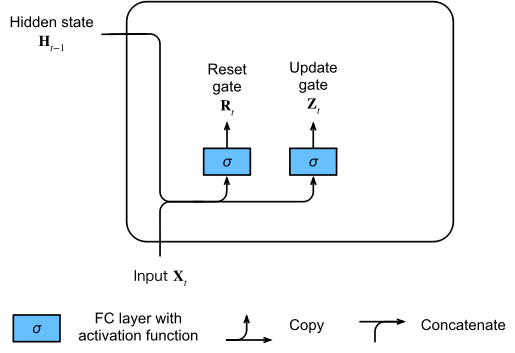
\includegraphics[scale=0.8]{gru-1.png}
  \hspace{1in}
  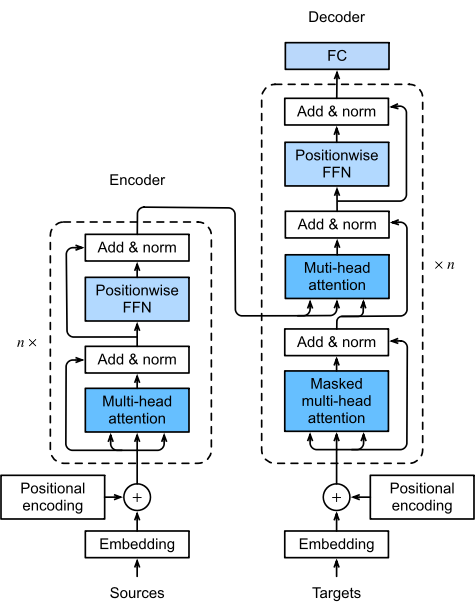
\includegraphics[scale=0.6]{transformer.png}
  \caption{GRU and Transformer}
\end{figure}
      \item \textbf{GRU} a gating mechanism in recurrent neural networks, the features extracted by CNN are input into the GRU layer. In practical attempts, GRU can be replaced with other sequence models such as RNN, LSTM and its variants to improve performance.
       \\ \hspace*{\fill} \\
      \item \textbf{Transformer} Compared with the GRU model, the Transformer uses a self-attention mechanism to differentially weight the importance of each part of the input data, and performs best in our experiments
    \end{itemize}

  \end{alertblock}

\end{column}

\separatorcolumn

\begin{column}{\colwidth}

  \begin{block}{Models}
    \textmd{After preprocessing the data image, the input consists of a feature extraction layer, which consists of multiple nonlinear functions and pooling layers. The nonlinear function functions include correlation coefficient, maximum value, minimum value, etc. The convolution kernels in CNN are consistent . Two feature extraction layers are used in our model, and the functions of the two layers have different lookback intervals (10 days and 5 days).}
    \\ \hspace*{\fill} \\
    \textmd{The extracted features are input to the pooling layer and the output is flattened and input to the recurrent neural network layer. Finally, the fully connected layer is input to obtain the prediction result. The parameters of the entire network will be optimized by back-propagation according to the loss of the prediction target. The role of the fully connected layer is to perform weighted synthesis of features, which is consistent with the fully connected layer in CNN.}
    \begin{table}
      \centering
      \begin{tabular}{l c}
        \toprule
        \textbf{Name} & \textbf{Definition} \\
        \midrule
        $corr(X, Y, d)$ & Correlation coefficient between the series $X$ and $Y$ for the past $d$ days\\
        $return(X, d)$ & $(X - delay(X, d))/delay(X, d)-1$, $delay(X, d)$ is $X$ over the past $d$ days\\
        $zscore(X, d)$ & The mean divided by the standard deviation of $X$ over the past $d$ days\\
        $min(X, d)$ & The minimum value of $X$ over the past $d$ days \\
        $...$&$...$\\
        \bottomrule
      \end{tabular}
      \caption{Functions in Feature Extraction Layer}
    \end{table}

\begin{figure}[htbp]
\leftline{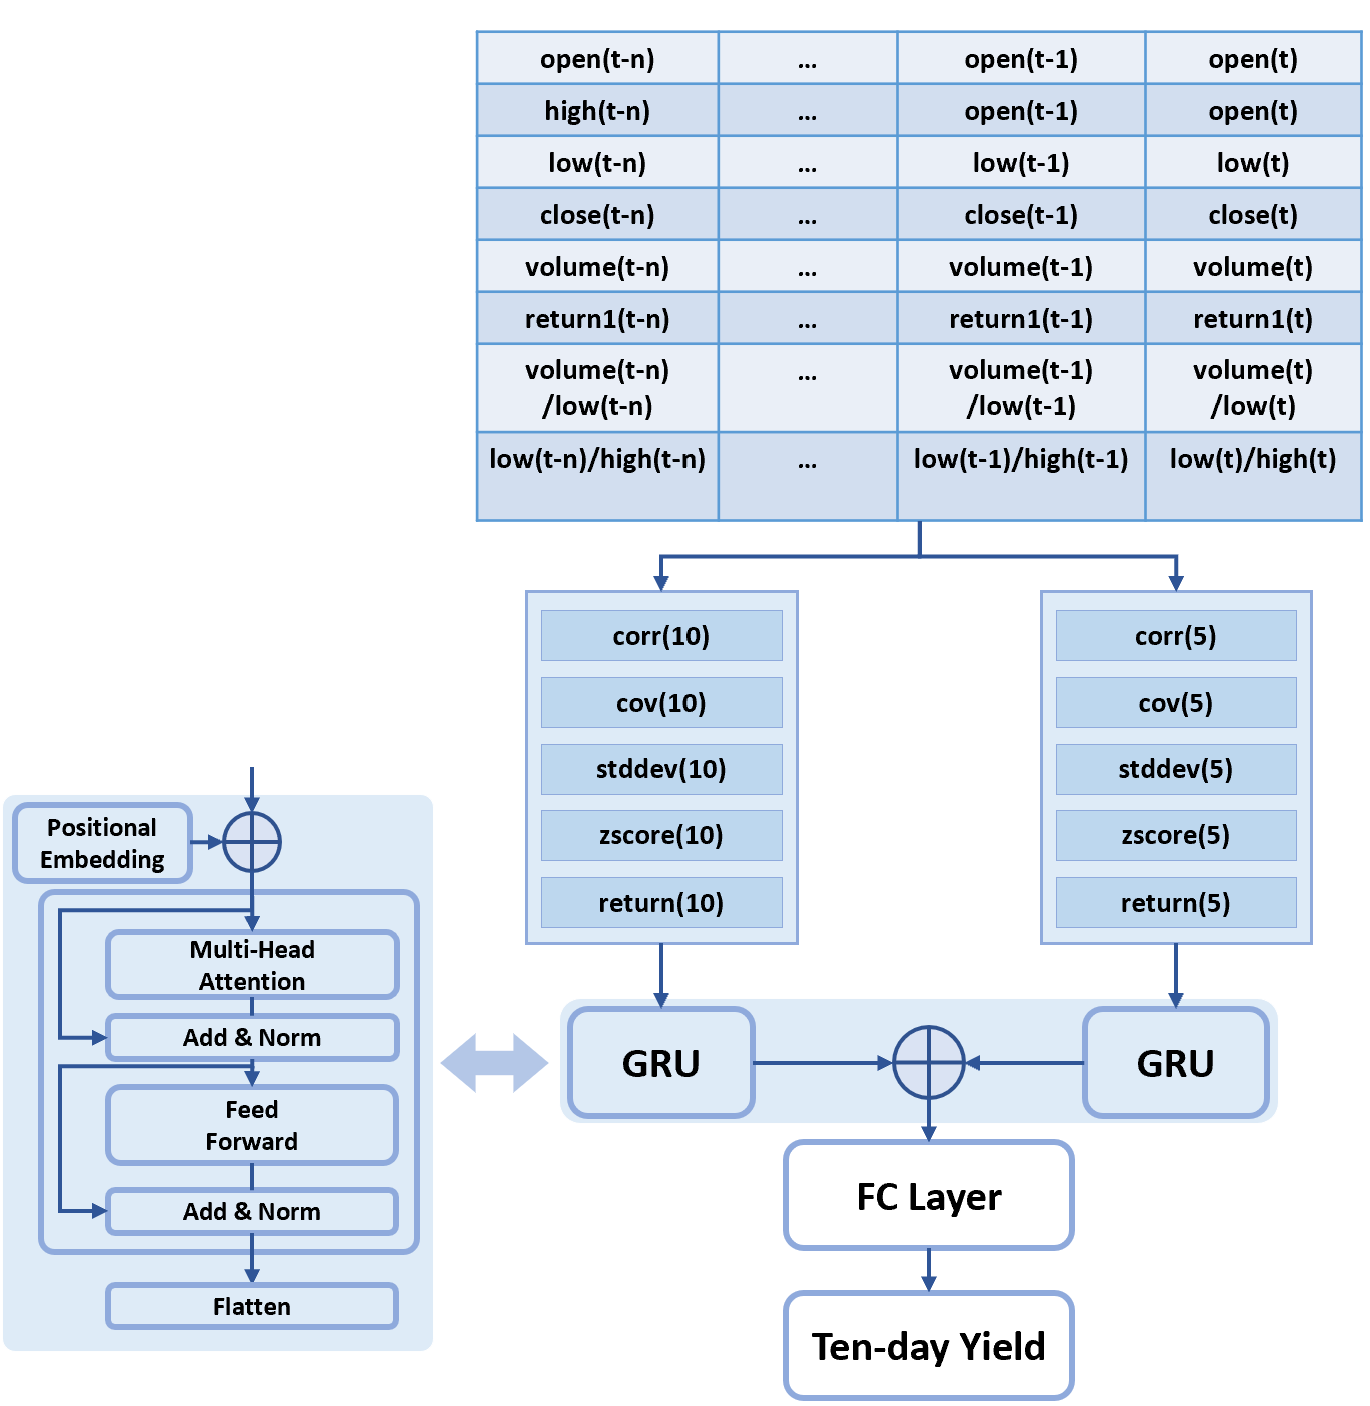
\includegraphics[width=0.9\linewidth]{model.png}}
    \caption{The structure of model}
    \label{fig:model}
\end{figure}

  \end{block}


\end{column}

\separatorcolumn

\begin{column}{\colwidth}

  \begin{exampleblock}{Results}
    We have trained on multiple stocks. The selected training set starts from July 2015, and the test set starts from January 2021. The following figure shows the prediction results of the stocks Tesla and Facebook. It can be seen that using transformers The model is better at predicting both trends and concrete values than the model using GRU. We tested an average RMSE of 0.0329 for the transformer module and 0.1138 for the GRU module.
    \begin{figure}
  \centering
  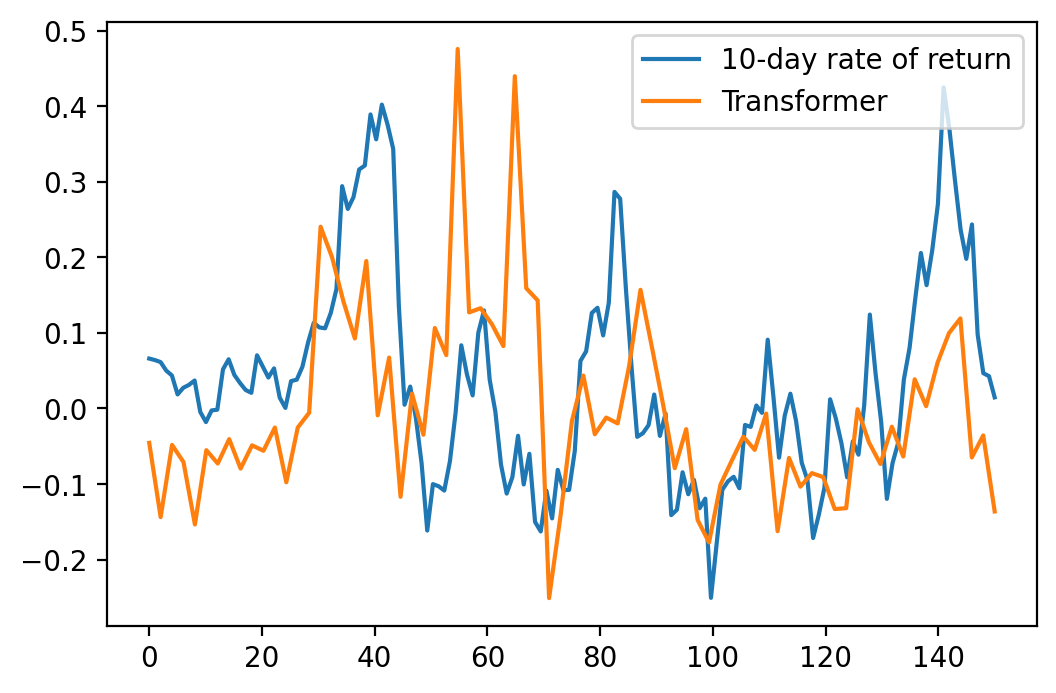
\includegraphics[scale=1]{out1.png}
  \hspace{1in}
  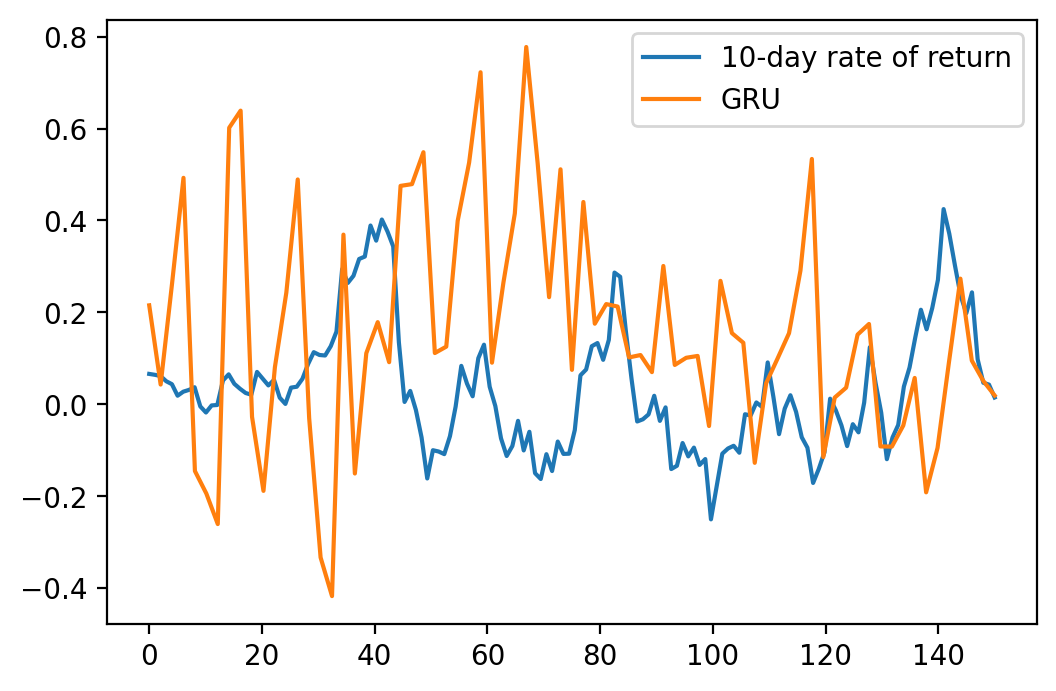
\includegraphics[scale=1]{outg.png}
  \caption{Test results using Transformer and GRU, starting on 2021/01/08}
\end{figure}
    \begin{figure}
  \centering
  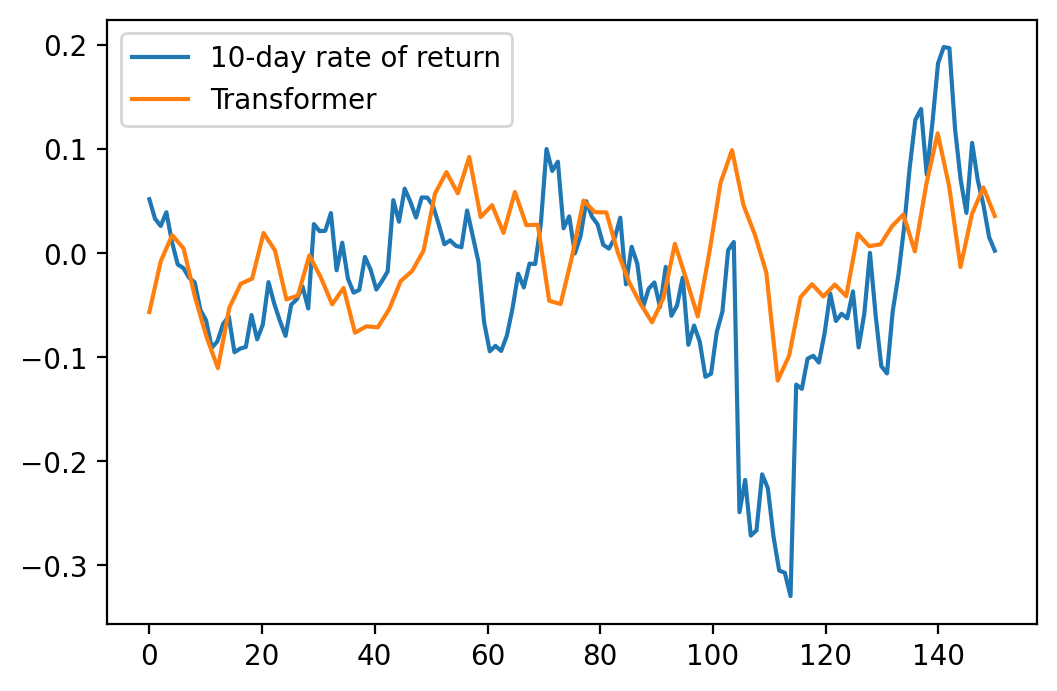
\includegraphics[scale=1]{outft.png}
  \hspace{1in}
  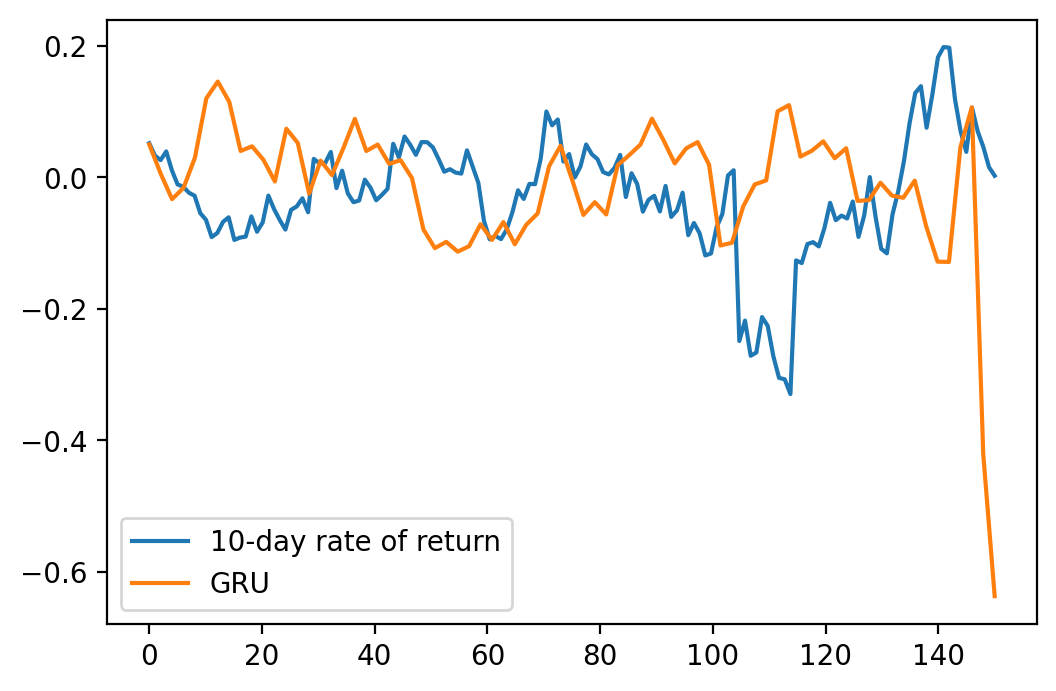
\includegraphics[scale=1]{outputfg.png}
  \caption{Test results using Transformer and GRU, starting on 2021/07/12}
  
\end{figure}
\begin{figure}[H]
\begin{minipage}{0.48\linewidth}
 \rightline{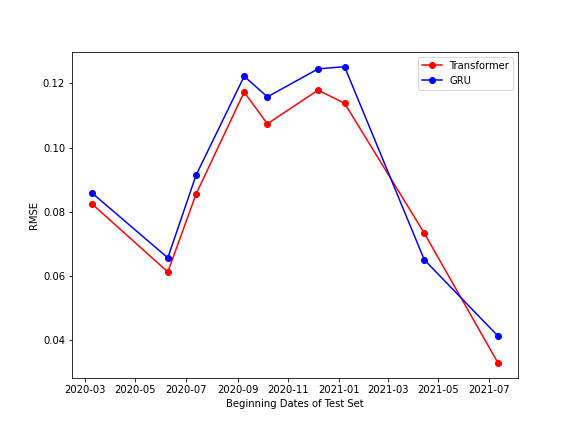
\includegraphics[width=14.5cm]{rmse.PNG}}
\end{minipage}
\hfill
\begin{minipage}{.48\linewidth}
\begin{table}
      \begin{tabular}{l r c}
        \toprule
        \textbf{Test set} & \textbf{Model} & \textbf{RMSE}\\
        \midrule
        2021/1 & Transformer & 0.1138 \\
        2021/1 & GRU & 0.1252 \\
        2021/7 & Transformer & 0.0329 \\
        2021/7 & GRU & 0.0413 \\
        \bottomrule
      \end{tabular}
    \end{table}
\end{minipage}
\caption{RMSE}
\end{figure}

  \end{exampleblock}

  \begin{block}{Evaluation}

    Compared with the common genetic programming + random forest model in the industry.
    
    \textbf{Advantages}
    
    1. End-to-end learning, optimized using the same objective function
    
    2. Training process is simplified without manual intervention, avoiding the work of selecting features
    
    \textbf{Disadvantages}
    
    1. The model interpretability is low.
    
    2. The feature extraction layer that can be embedded in the neural network is still relatively limited, and the factor calculation method cannot be updated in practical applications.
  \end{block}
\end{column}

\separatorcolumn
\end{columns}
\end{frame}

\end{document}
